\chapter{Bâtons Salés}
\label{ch:batonsale}
\index{dessert}
\index{cookie}

\marginnote{
    \textbf{Makes 40-60 cookies} \\
    Prep time: 45 minutes \\
    Cook time: 30 minutes \\
    \vspace*{\baselineskip}

    5 cups all-purpose flour \\
    3 tsp baking powder \\
    1 tsp salt \\
    1 cup warm water \\
    1 1/2 cups vegetable oil \\
    1/2 cup zaatar \\
    1 egg \\
    Nigella seeds
}

\textit{Savoury sticks}

Family member: Nene Hermine

\begin{enumerate}
    \item In a large bowl, mix all the ingredients except the egg and nigella seeds. Add an additional flour if needed to obtain a non-sticky soft yet pliable dough.
    \item Shape into 4-5 inch thin ropes. Fold each rope in half then form a twisted rope.
    \item Place on baking sheet lined with parchment.
    \item Lightly brush with egg wash and sprinkle with nigella seeds.
    \item Bake at 350\degree F for about 30 minutes.
\end{enumerate}

Sybil’s trick: You can freeze 2/3 of the cookies once they have baked and cooled.

% Find right place for pictures
% \begin{figure}
  % 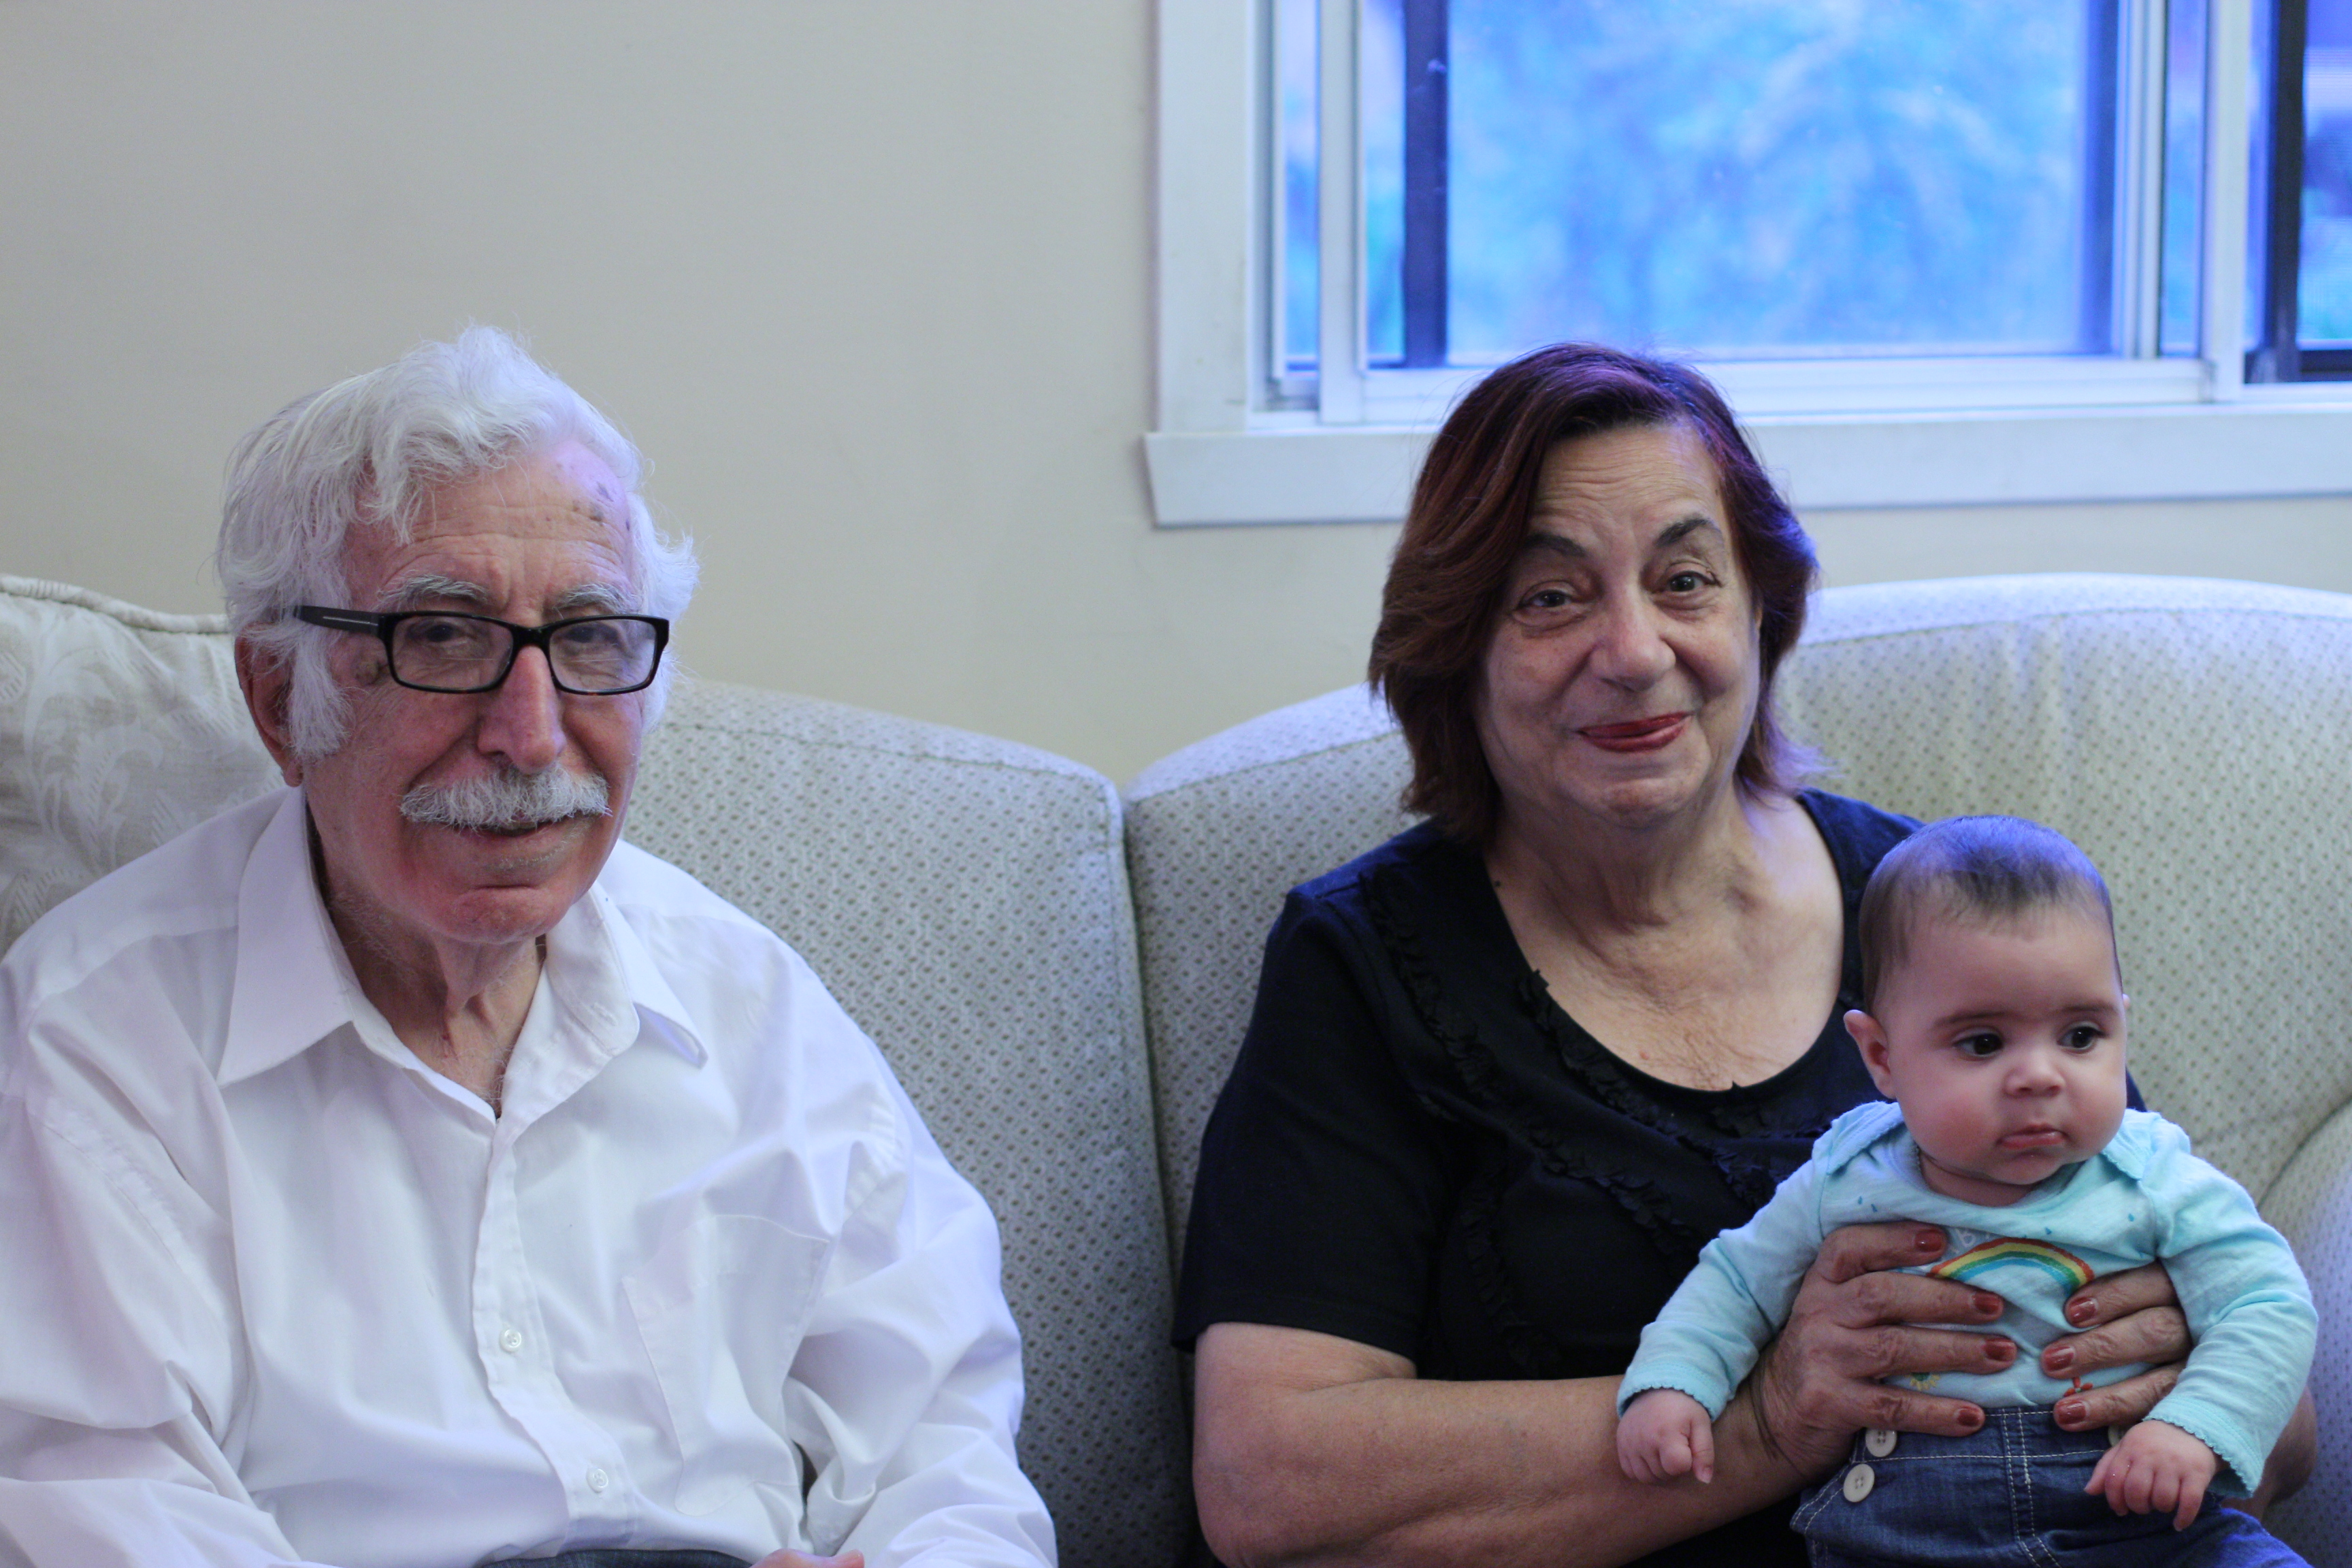
\includegraphics[width=60mm]{dermardiros/images/Grandpa and grandma.JPG}
  % 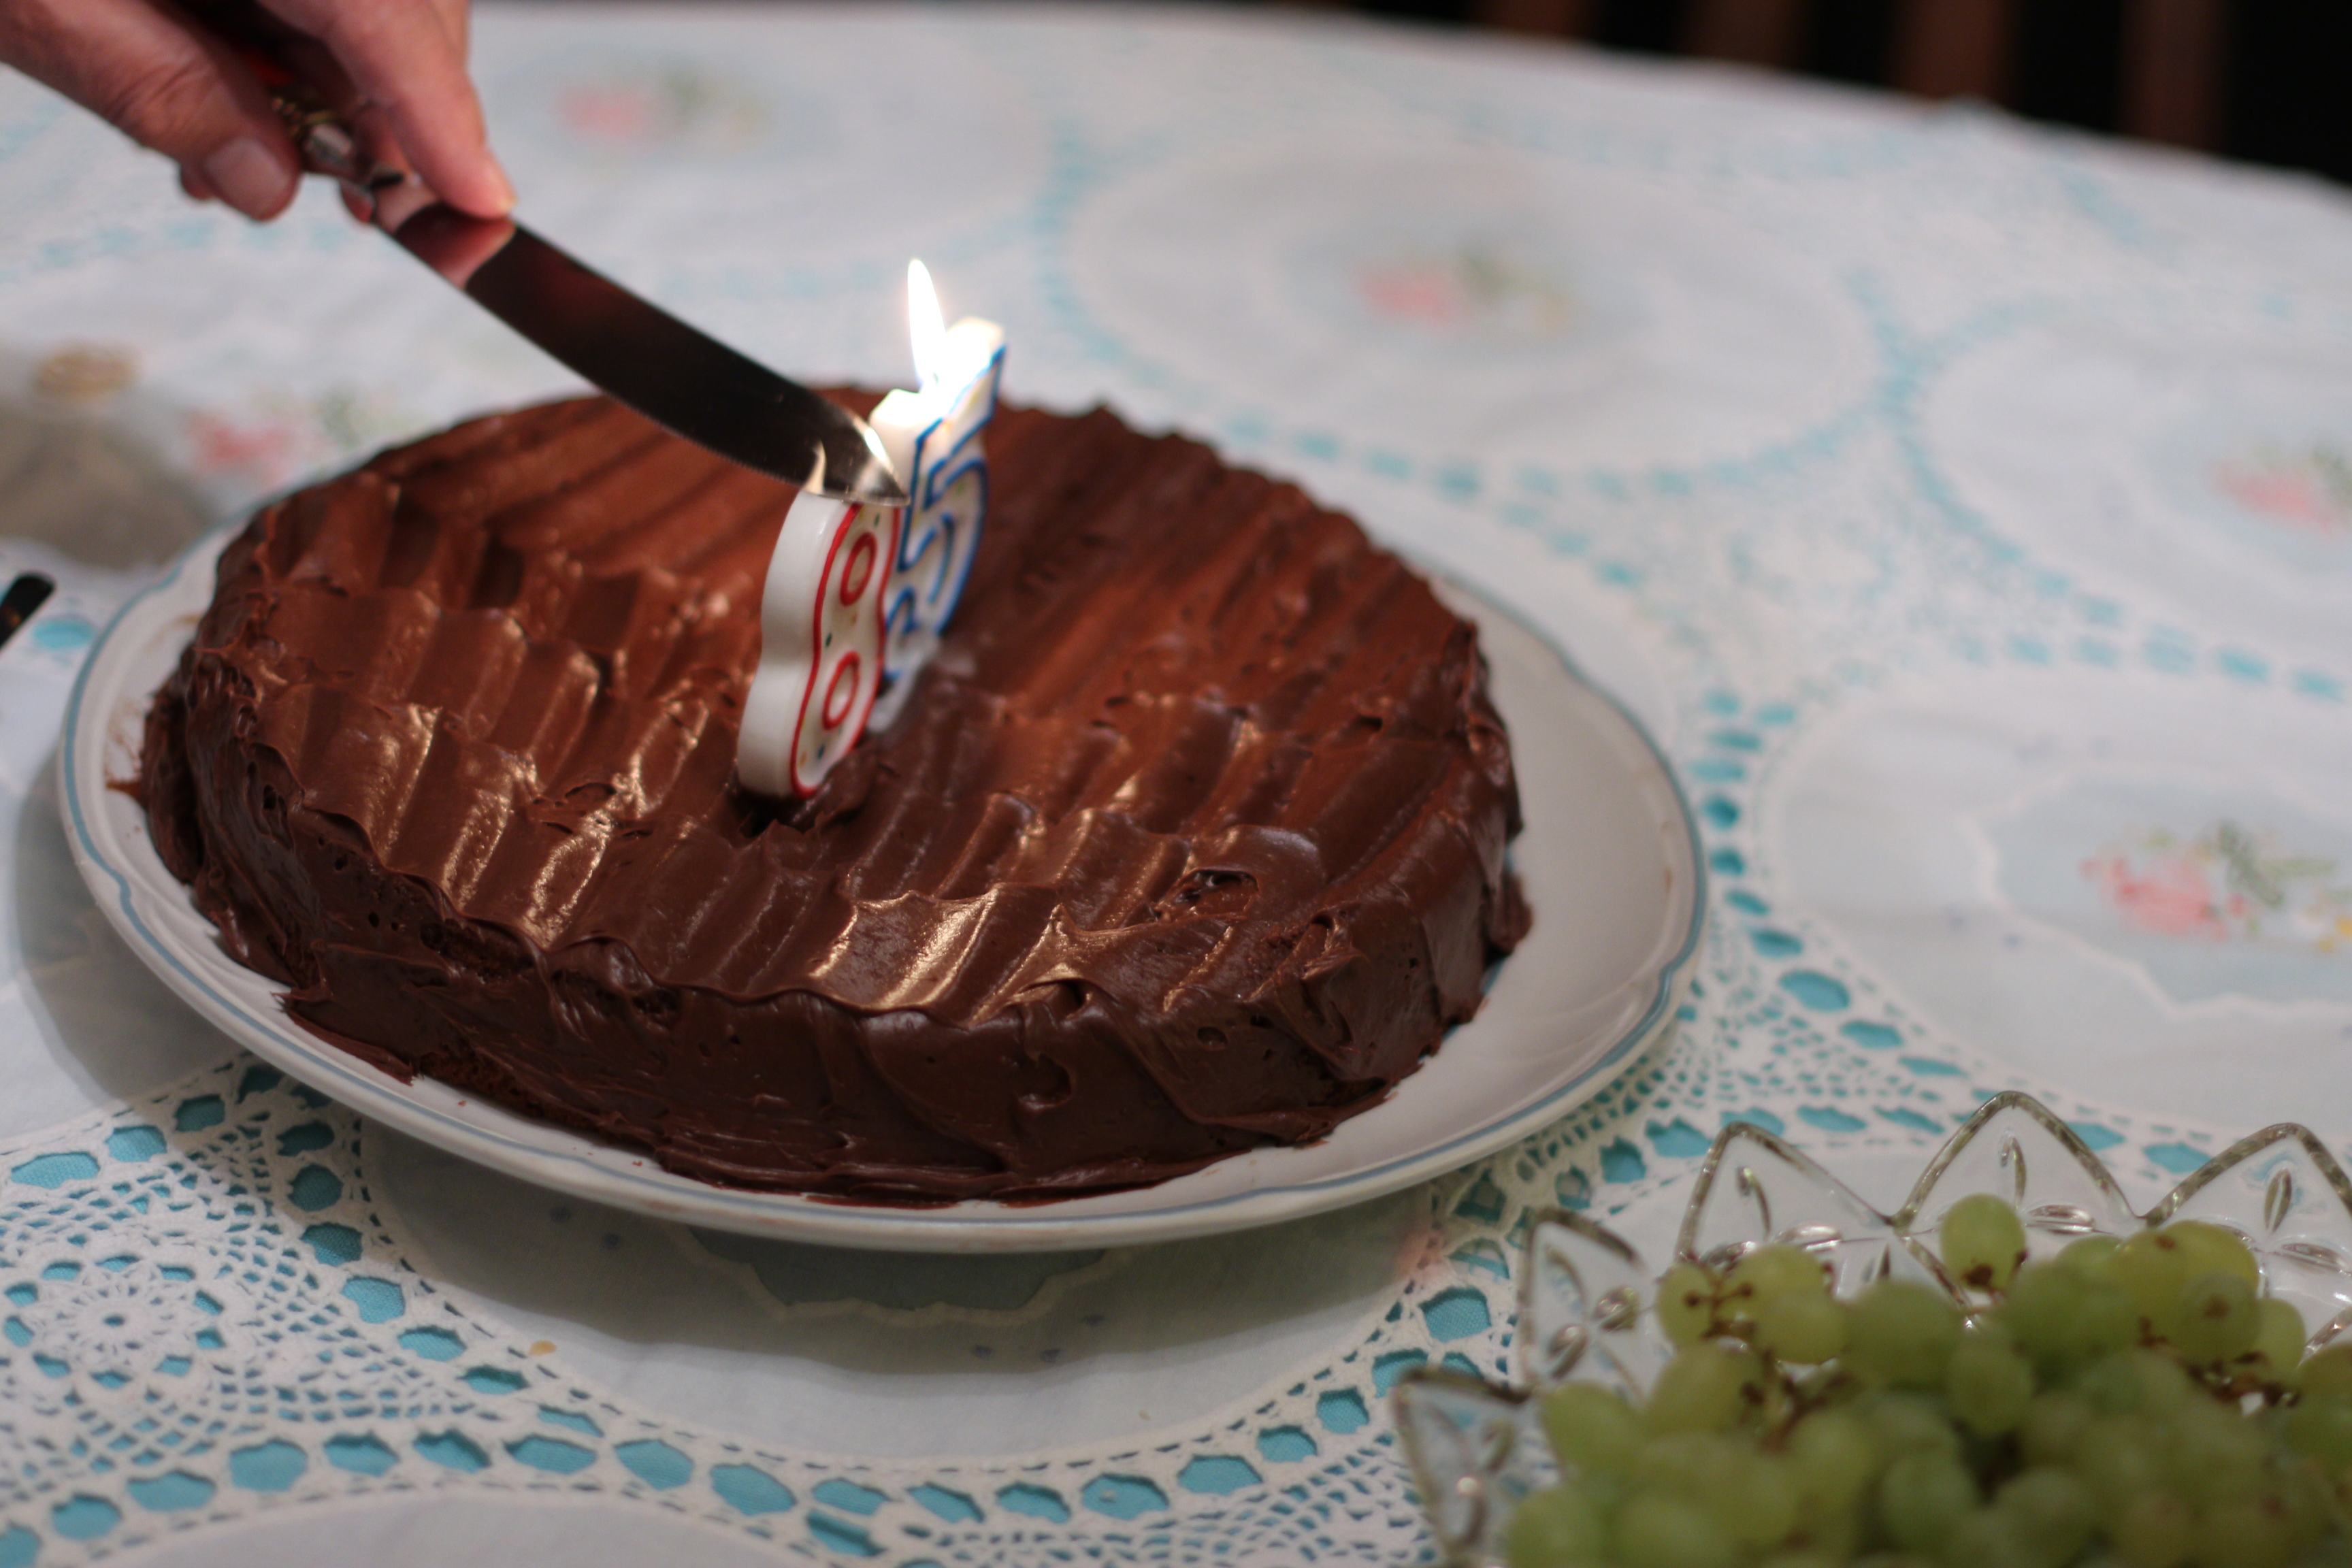
\includegraphics[width=60mm]{dermardiros/images/Grandpa and Grandma 2.JPG}
  % \includegraphics[width=60mm]{dermardiros/images/Grandpa and Grandma 3.png}
% \end{figure}
